
%(BEGIN_QUESTION)
% Copyright 2006, Tony R. Kuphaldt, released under the Creative Commons Attribution License (v 1.0)
% This means you may do almost anything with this work of mine, so long as you give me proper credit

Calculate the 0\%, 50\%, and 100\% calibration points for the $\Delta$P transmitter to measure liquid level in this vessel, given a range of 0 to 30 feet and a process specific gravity of 0.85.  Note the ``wet'' leg filled with fluid different than the process (SG = 1.1), 35 feet tall:

$$\includegraphics[width=15.5cm]{i00263x01.eps}$$

% No blank lines allowed between lines of an \halign structure!
% I use comments (%) instead, so that TeX doesn't choke.

$$\vbox{\offinterlineskip
\halign{\strut
\vrule \quad\hfil # \ \hfil & 
\vrule \quad\hfil # \ \hfil & 
\vrule \quad\hfil # \ \hfil \vrule \cr
\noalign{\hrule}
%
% First row
\% of span & $\Delta$P ("H$_{2}$O) & Output (mA) \cr
%
\noalign{\hrule}
%
% Another row
0 &  &  \cr
%
\noalign{\hrule}
%
% Another row
50 &  &  \cr
%
\noalign{\hrule}
%
% Another row
100 &  &  \cr
%
\noalign{\hrule}
} % End of \halign 
}$$ % End of \vbox

\underbar{file i00263}
%(END_QUESTION)





%(BEGIN_ANSWER)

% No blank lines allowed between lines of an \halign structure!
% I use comments (%) instead, so that TeX doesn't choke.

$$\vbox{\offinterlineskip
\halign{\strut
\vrule \quad\hfil # \ \hfil & 
\vrule \quad\hfil # \ \hfil & 
\vrule \quad\hfil # \ \hfil \vrule \cr
\noalign{\hrule}
%
% First row
\% of span & $\Delta$P ("H$_{2}$O) & Output (mA) \cr
%
\noalign{\hrule}
%
% Another row
0 & -462 & 10 \cr
%
\noalign{\hrule}
%
% Another row
50 & -309 & 30 \cr
%
\noalign{\hrule}
%
% Another row
100 & -156 & 50 \cr
%
\noalign{\hrule}
} % End of \halign 
}$$ % End of \vbox

%(END_ANSWER)





%(BEGIN_NOTES)


%INDEX% Measurement, level: hydrostatic pressure (elevated zero)
%INDEX% Measurement, level: hydrostatic pressure (``wet'' reference leg)

%(END_NOTES)


